\chapter{Dimensionnement analytique}
\label{ch-dim}

Ce chapitre correspond à l'Étape 1 du sujet. Tous les résultats sont produits par notre script de calcul à partir du tableau d'hypothèses du \cref{ch-cdc}.

\section{Les marges}
\label{sec-marges}

\subsection{Effet de masque et probabilité de couverture}

Autour de la valeur moyenne donnée par le modèle de propagation, le niveau reçu varie d'un point à l'autre à cause du relief et des bâtiments. Cette variation, l'effet de masque, suit une loi log-normale : en décibels, une loi normale d'écart-type $\sigma$~\cite{rappaport2002}. Nous retenons $\sigma = \SI{8}{\deci\bel}$ en ville et $\sigma = \SI{6}{\deci\bel}$ en campagne, valeurs usuelles pour ces milieux.

L'objectif porte sur \SI{95}{\percent} de la \emph{surface} de la cellule. Le bord est le point le plus défavorable, donc une probabilité plus faible y suffit. La formule de Jakes~\cite{jakes1974} relie les deux probabilités :
\begin{equation}
  F_u = \frac{1}{2}\left[1 - \operatorname{erf}(a) + \exp\!\left(\frac{1 - 2ab}{b^2}\right)\left(1 - \operatorname{erf}\!\left(\frac{1 - ab}{b}\right)\right)\right],
  \qquad a = \frac{-M}{\sigma\sqrt{2}}, \quad b = \frac{10\,n\log_{10} e}{\sigma\sqrt{2}},
  \label{eq-jakes}
\end{equation}
où $F_u$ est la fraction de la surface couverte, $M$ la marge au bord de la cellule et $n$ l'exposant d'affaiblissement. Avec le modèle de Hata (\cref{sec-hata}), la pente vaut $44{,}9 - 6{,}55\log_{10} 30 = \SI{35,2}{\deci\bel}$ par décade, soit $n = 3{,}52$. La résolution de l'équation~\eqref{eq-jakes} pour $F_u = \SI{95}{\percent}$ donne le \cref{tab-jakes}.

\begin{table}[H]
\centering
\caption{Marges d'effet de masque (Jakes, $n = 3{,}52$).}
\label{tab-jakes}
\begin{tabular}{@{}lccccc@{}}
\toprule
\thead{Zone} & \thead{$\sigma$ (dB)} & \thead{$b$} & \thead{$a$} & \thead{Probabilité au bord} & \thead{Marge (dB)} \\
\midrule
Urbain & 8 & 1,352 & $-0{,}767$ & \SI{86,1}{\percent} & \textbf{8,7} \\
Rural & 6 & 1,803 & $-0{,}690$ & \SI{83,5}{\percent} & \textbf{5,9} \\
\bottomrule
\end{tabular}
\end{table}

\begin{figure}[H]
\centering
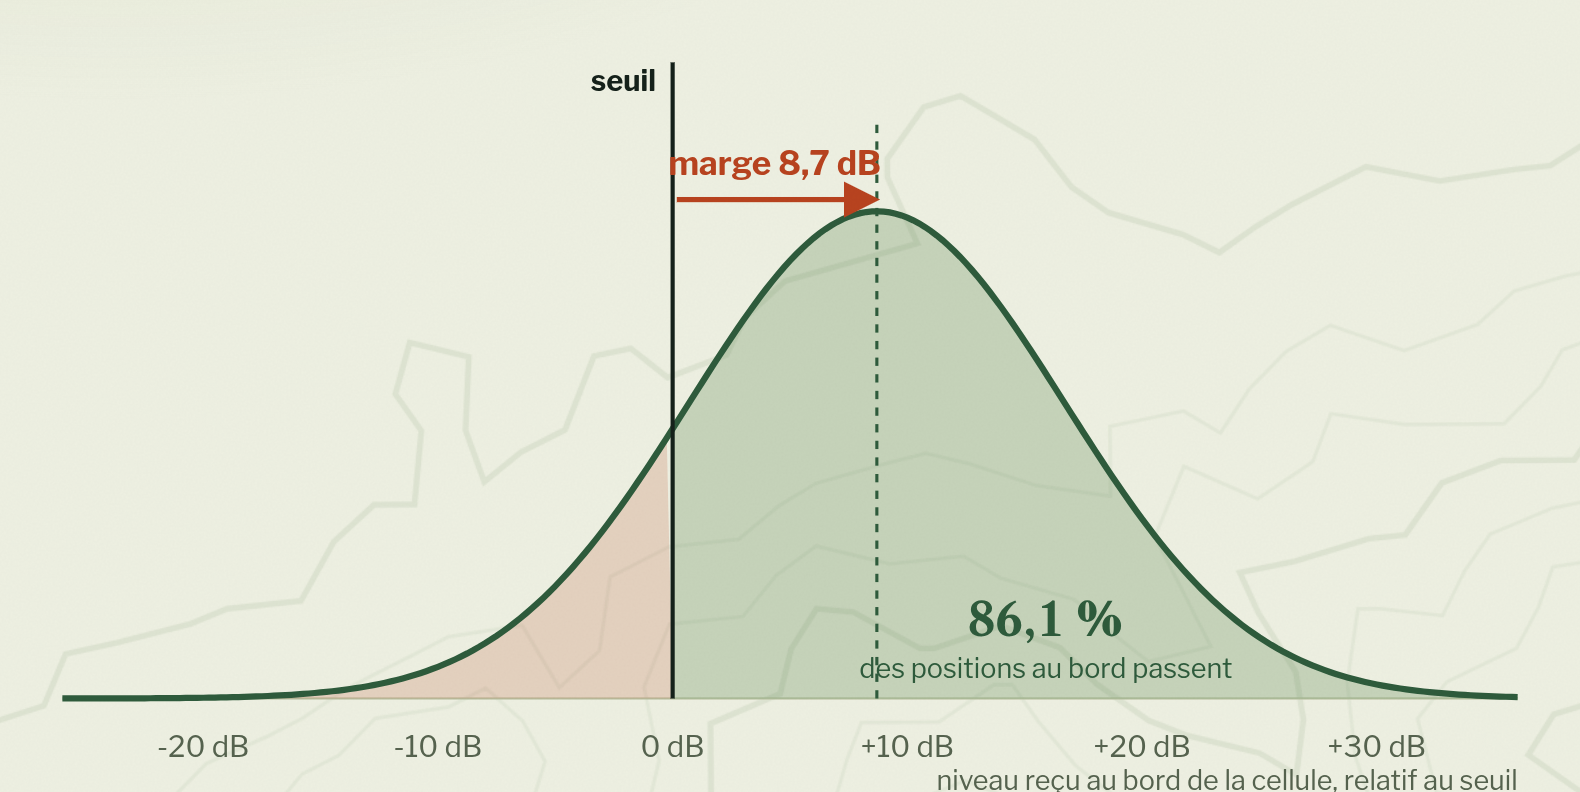
\includegraphics[width=0.72\textwidth]{marges-gauss.png}
\caption{Marge d'effet de masque au bord d'une cellule urbaine.}
\label{fig-gauss}
\end{figure}

La \cref{fig-gauss} montre la distribution du niveau reçu au bord d'une cellule urbaine ($\sigma = \SI{8}{\deci\bel}$). Avec une moyenne \SI{8,7}{\deci\bel} au-dessus du seuil, \SI{86,1}{\percent} des positions du bord sont couvertes, et donc \SI{95}{\percent} de la surface.

\subsection{Les autres marges}

La pénétration dans les bâtiments est de \SI{15}{\deci\bel} pour le bâti dense à \SI{1800}{\mega\hertz} et de \SI{10}{\deci\bel} pour les autres classes ; elle ne s'applique qu'à l'objectif indoor de la ville. La marge d'interférence est de \SI{2}{\deci\bel} en UL et \SI{3}{\deci\bel} en DL, pour tenir compte de la charge des cellules voisines en réutilisation~1.

\begin{cours}{évanouissements rapides}
La prise en compte du fading de Rayleigh impose des marges de fading de 10 à \SI{15}{\deci\bel}~\cite{afif2026cours}.
\application Nous prenons une marge de \SI{0}{\deci\bel}. Le cours raisonne sur un système FDMA à bande étroite. En LTE, les seuils de SINR des bearers d'Atoll sont issus de simulations au niveau du lien qui intègrent déjà le canal à évanouissements, la diversité et les retransmissions~\cite{holma2011}, et Atoll n'ajoute aucune marge de ce type. Ajouter \SI{10}{\deci\bel} compterait le phénomène deux fois : le rayon urbain passerait de \SI{0,64}{\kilo\metre} à \SI{0,33}{\kilo\metre}, soit environ 3,7 fois plus de sites.
\end{cours}

\section{Le bilan de liaison}
\label{sec-bilan}

\begin{cours}{bilan de liaison}
La frontière d'une cellule est l'ensemble des points où un mobile de la plus faible puissance autorisée peut communiquer avec sa station \emph{dans les deux sens}. Les liaisons montante et descendante doivent être équilibrées~\cite{afif2026cours}.
\application Nous calculons les deux bilans et retenons le plus contraignant. L'utilisateur de bord de cellule est servi au bearer~4 (SINR $\geq \SI{-1}{\deci\bel}$) ; il lui faut 2 RB pour \SI{128}{\kbps} en UL et 15 RB pour \SI{1024}{\kbps} en DL.
\end{cours}

\paragraph{Sensibilité.} La sensibilité du récepteur de la station en UL, sur 2 RB (\SI{360}{\kilo\hertz}), vaut
\begin{equation}
  S = \underbrace{-174 + 10\log_{10}(\num{360e3})}_{\text{bruit thermique : } -118{,}4} + \underbrace{5}_{\text{NF}} \; \underbrace{-\,1}_{\text{SINR}} = \SI{-114,4}{\dBm}.
\end{equation}

\paragraph{Affaiblissement maximal (MAPL).} L'affaiblissement de parcours maximal admissible est la somme algébrique des gains, des pertes et des marges :
\begin{equation}
  \text{MAPL} = P_{\text{UE}} + G_{\text{eNB}} - L_{\text{eNB}} - S - M_{\text{masque}} - M_{\text{interf}} - L_{\text{indoor}} - M_{\text{fading}}.
  \label{eq-mapl}
\end{equation}

\begin{table}[H]
\centering
\caption{Bilan de liaison du centre urbain (indoor, tri-secteur).}
\label{tab-bilan}
\small
\begin{tabular}{@{}lr@{\hspace{1.6em}}lr@{}}
\toprule
\thead{Liaison montante (UL)} & & \thead{Liaison descendante (DL)} & \\
\midrule
Puissance du terminal & \SI{23,0}{\dBm} & Puissance eNB par RB (\SI{46}{\dBm} / 100) & \SI{26,0}{\dBm} \\
Gain antenne eNB $-$ pertes & \SI{17,0}{\deci\bel} & Gain antenne $-$ pertes & \SI{17,0}{\deci\bel} \\
Sensibilité eNB (2 RB) & \SI{-114,4}{\dBm} & Sensibilité terminal (1 RB) & \SI{-114,5}{\dBm} \\
Marge de masque & \SI{-8,7}{\deci\bel} & Marge de masque & \SI{-8,7}{\deci\bel} \\
Marge d'interférence & \SI{-2,0}{\deci\bel} & Marge d'interférence & \SI{-3,0}{\deci\bel} \\
Pénétration indoor & \SI{-15,0}{\deci\bel} & Pénétration indoor & \SI{-15,0}{\deci\bel} \\
Évanouissement rapide & \SI{0}{\deci\bel} & Évanouissement rapide & \SI{0}{\deci\bel} \\
\midrule
\textbf{MAPL} & \textbf{\SI{128,8}{\deci\bel}} & \textbf{MAPL} & \textbf{\SI{130,8}{\deci\bel}} \\
\bottomrule
\end{tabular}
\end{table}

La liaison montante est limitante de \SI{2,0}{\deci\bel}, en ville comme en campagne (MAPL rural : \SI{146,6}{\deci\bel} en UL contre \SI{148,6}{\deci\bel} en DL), car la station émet \SI{46}{\dBm} et le terminal seulement \SI{23}{\dBm}. Un écart de \SI{2}{\deci\bel} reste faible : le bilan est presque équilibré, comme le demande le cours. La PIRE de la station vaut $46 + 18 - 1 = \SI{63}{\dBm}$.

\begin{figure}[H]
\centering
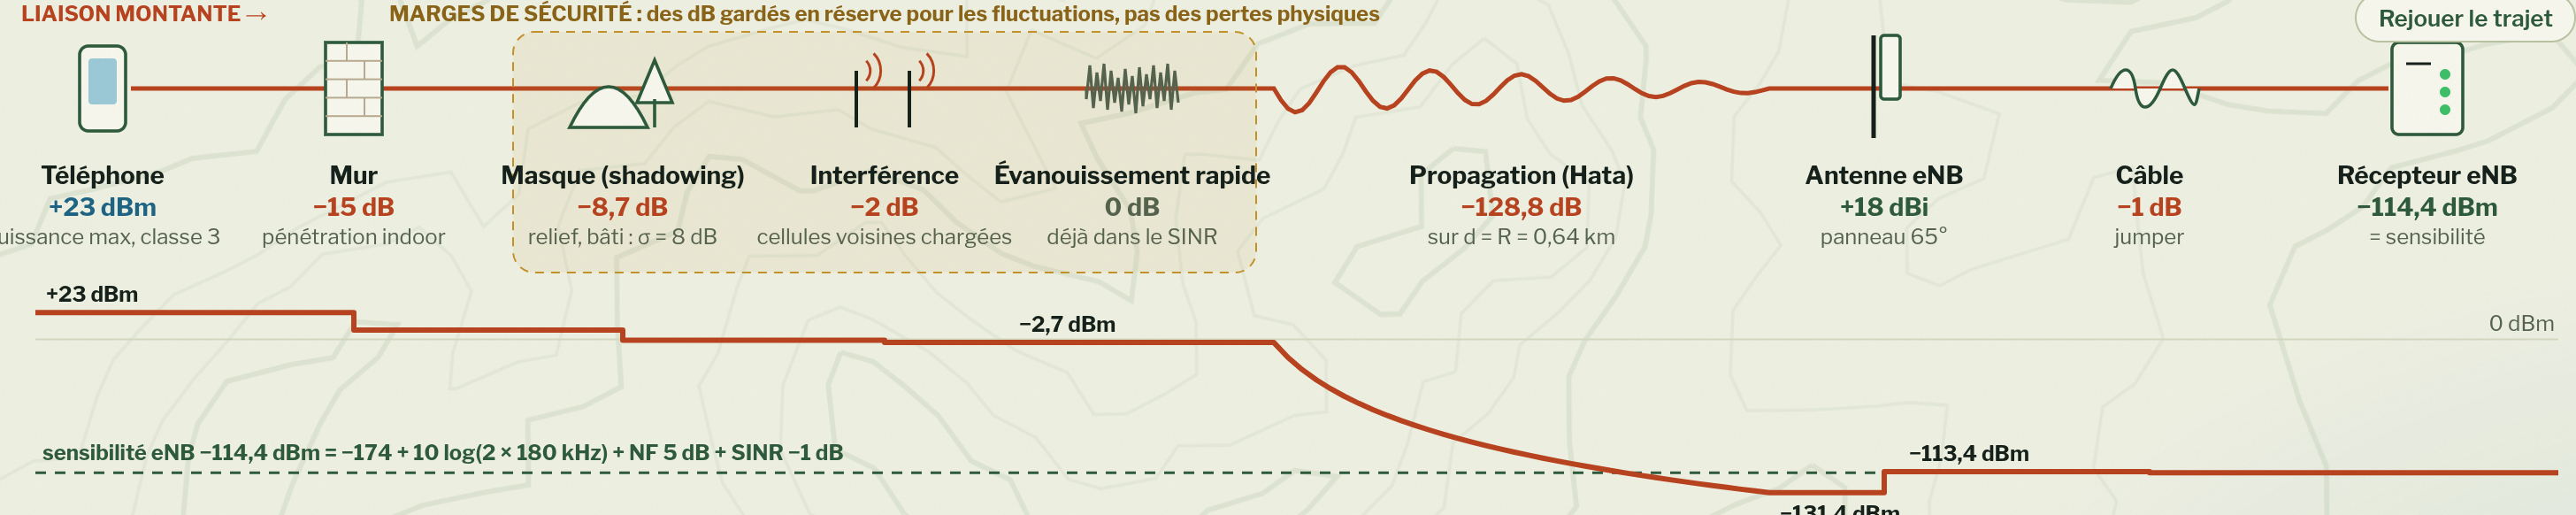
\includegraphics[width=\textwidth]{bilan-chaine.png}
\caption{Bilan de liaison montante, du terminal à la station.}
\label{fig-chaine}
\end{figure}

La \cref{fig-chaine} suit le signal du téléphone (\SI{+23}{\dBm}) jusqu'au récepteur de la station. Les marges (cadre pointillé) ne sont pas des pertes physiques mais des réserves pour les fluctuations ; à la distance $R$, le signal arrive exactement à la sensibilité de \SI{-114,4}{\dBm}.

\subsection{Le modèle de propagation et le rayon}
\label{sec-hata}

À \SI{1800}{\mega\hertz}, nous utilisons le modèle COST-231 Hata~\cite{cost231}, extension du modèle de Hata~\cite{hata1980} (lui-même tiré des mesures d'Okumura~\cite{okumura1968}) à la plage \SIrange{1500}{2000}{\mega\hertz} :
\begin{equation}
  L = 46{,}3 + 33{,}9\log_{10} f - 13{,}82\log_{10} h_b - a(h_m) + (44{,}9 - 6{,}55\log_{10} h_b)\log_{10} d + C_m,
  \label{eq-hata}
\end{equation}
\begin{equation}
  a(h_m) = (1{,}1\log_{10} f - 0{,}7)\,h_m - (1{,}56\log_{10} f - 0{,}8),
\end{equation}
avec $f$ en \si{\mega\hertz}, $d$ en \si{\kilo\metre}, $h_b = \SI{30}{\metre}$, $h_m = \SI{1,5}{\metre}$ et $C_m = \SI{0}{\deci\bel}$ (ville moyenne). À $f = \SI{1720}{\mega\hertz}$ (UL), on obtient $a(h_m) = \SI{0,04}{\deci\bel}$, $L(\SI{1}{\kilo\metre}) = \SI{135,5}{\deci\bel}$ et une pente de \SI{35,2}{\deci\bel} par décade. Le rayon est la distance où l'affaiblissement atteint le MAPL :
\begin{align}
  R &= 10^{(\text{MAPL} - 135{,}5)/35{,}2}, \\
  R_{\text{urbain}} &= 10^{(128{,}8 - 135{,}5)/35{,}2} = \SI{0,64}{\kilo\metre},
  \qquad
  R_{\text{rural}} = 10^{(146{,}6 - 135{,}5)/35{,}2} = \SI{2,06}{\kilo\metre}.
\end{align}
La même formule \enquote{ville moyenne} est utilisée en campagne. C'est un choix prudent, et c'est aussi le réglage par défaut d'Atoll, qui applique cette variante à toutes les classes d'occupation du sol. Le modèle est validé pour $d \geq \SI{1}{\kilo\metre}$ ; le rayon urbain de \SI{0,64}{\kilo\metre} en est une légère extrapolation, que nous acceptons car Atoll utilise le même modèle et que l'écart reste dans l'incertitude de l'effet de masque.

\section{Nombre de sites par la couverture}
\label{sec-sites}

La surface couverte par un site vaut $A_{\text{site}} = k R^2$, avec $k = \tfrac{3\sqrt{3}}{2} \approx 2{,}6$ pour une cellule omnidirectionnelle hexagonale et $k = 1{,}95$ pour un site tri-sectoriel. Le nombre de sites est le rapport de la surface de la zone à celle d'un site. Le gain d'antenne entre dans le bilan, donc chaque configuration a son propre rayon (\cref{tab-sites}).

\begin{table}[H]
\centering
\caption{Sites nécessaires à la couverture selon l'antenne.}
\label{tab-sites}
\begin{tabular}{@{}lccccc@{}}
\toprule
\thead{Configuration} & \thead{$R$ urbain} & \thead{Sites urbains} & \thead{$R$ rural} & \thead{Sites ruraux} & \thead{Total} \\
\midrule
Omni, \SI{11}{\dBi} & \SI{0,41}{\kilo\metre} & 20 & \SI{1,30}{\kilo\metre} & 18 & 38 \\
\rowcolor{mousse!50} \textbf{Tri-secteur \ang{65}, \SI{18}{\dBi}} & \SI{0,64}{\kilo\metre} & \textbf{11} & \SI{2,06}{\kilo\metre} & \textbf{10} & \textbf{21} \\
6 secteurs \ang{33}, \SI{21}{\dBi} & \SI{0,78}{\kilo\metre} & 6 & \SI{2,51}{\kilo\metre} & 5 & 11 \\
\bottomrule
\end{tabular}
\end{table}

Pour la configuration retenue :
\begin{equation}
  N_{\text{urbain}} = \frac{8{,}57}{1{,}95 × 0{,}64^2} = 10{,}7 \;\rightarrow\; 11,
  \qquad
  N_{\text{rural}} = \frac{76{,}95}{1{,}95 × 2{,}06^2} = 9{,}3 \;\rightarrow\; 10.
\end{equation}
La configuration à six secteurs demande moins de sites, mais 66 cellules au lieu de 63 et beaucoup plus de recouvrement en réutilisation~1. Nous gardons le tri-secteur, qui est la configuration recommandée par le cours (un site unique couvre trois cellules avec des antennes sectorielles, pour réduire le nombre de sites à installer et à gérer~\cite{afif2026cours}) et celle des modèles standard d'Atoll.

\begin{figure}[H]
\centering
\begin{subfigure}[b]{0.36\textwidth}\centering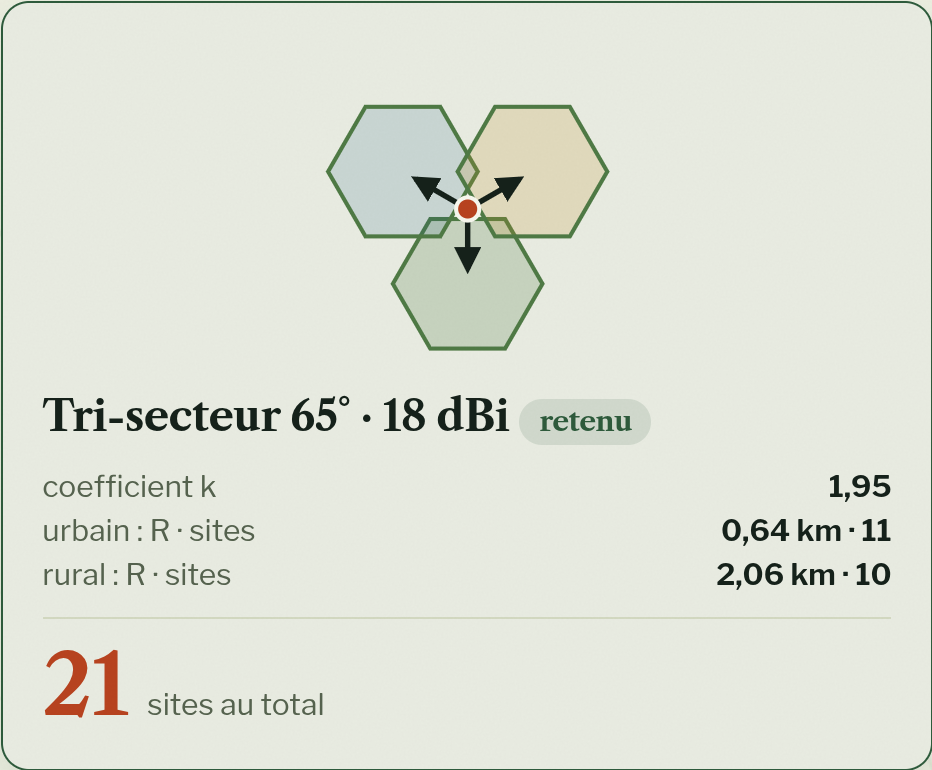
\includegraphics[width=\textwidth]{site-tri.png}\caption{Schéma du site.}\end{subfigure}\hfill
\begin{subfigure}[b]{0.6\textwidth}\centering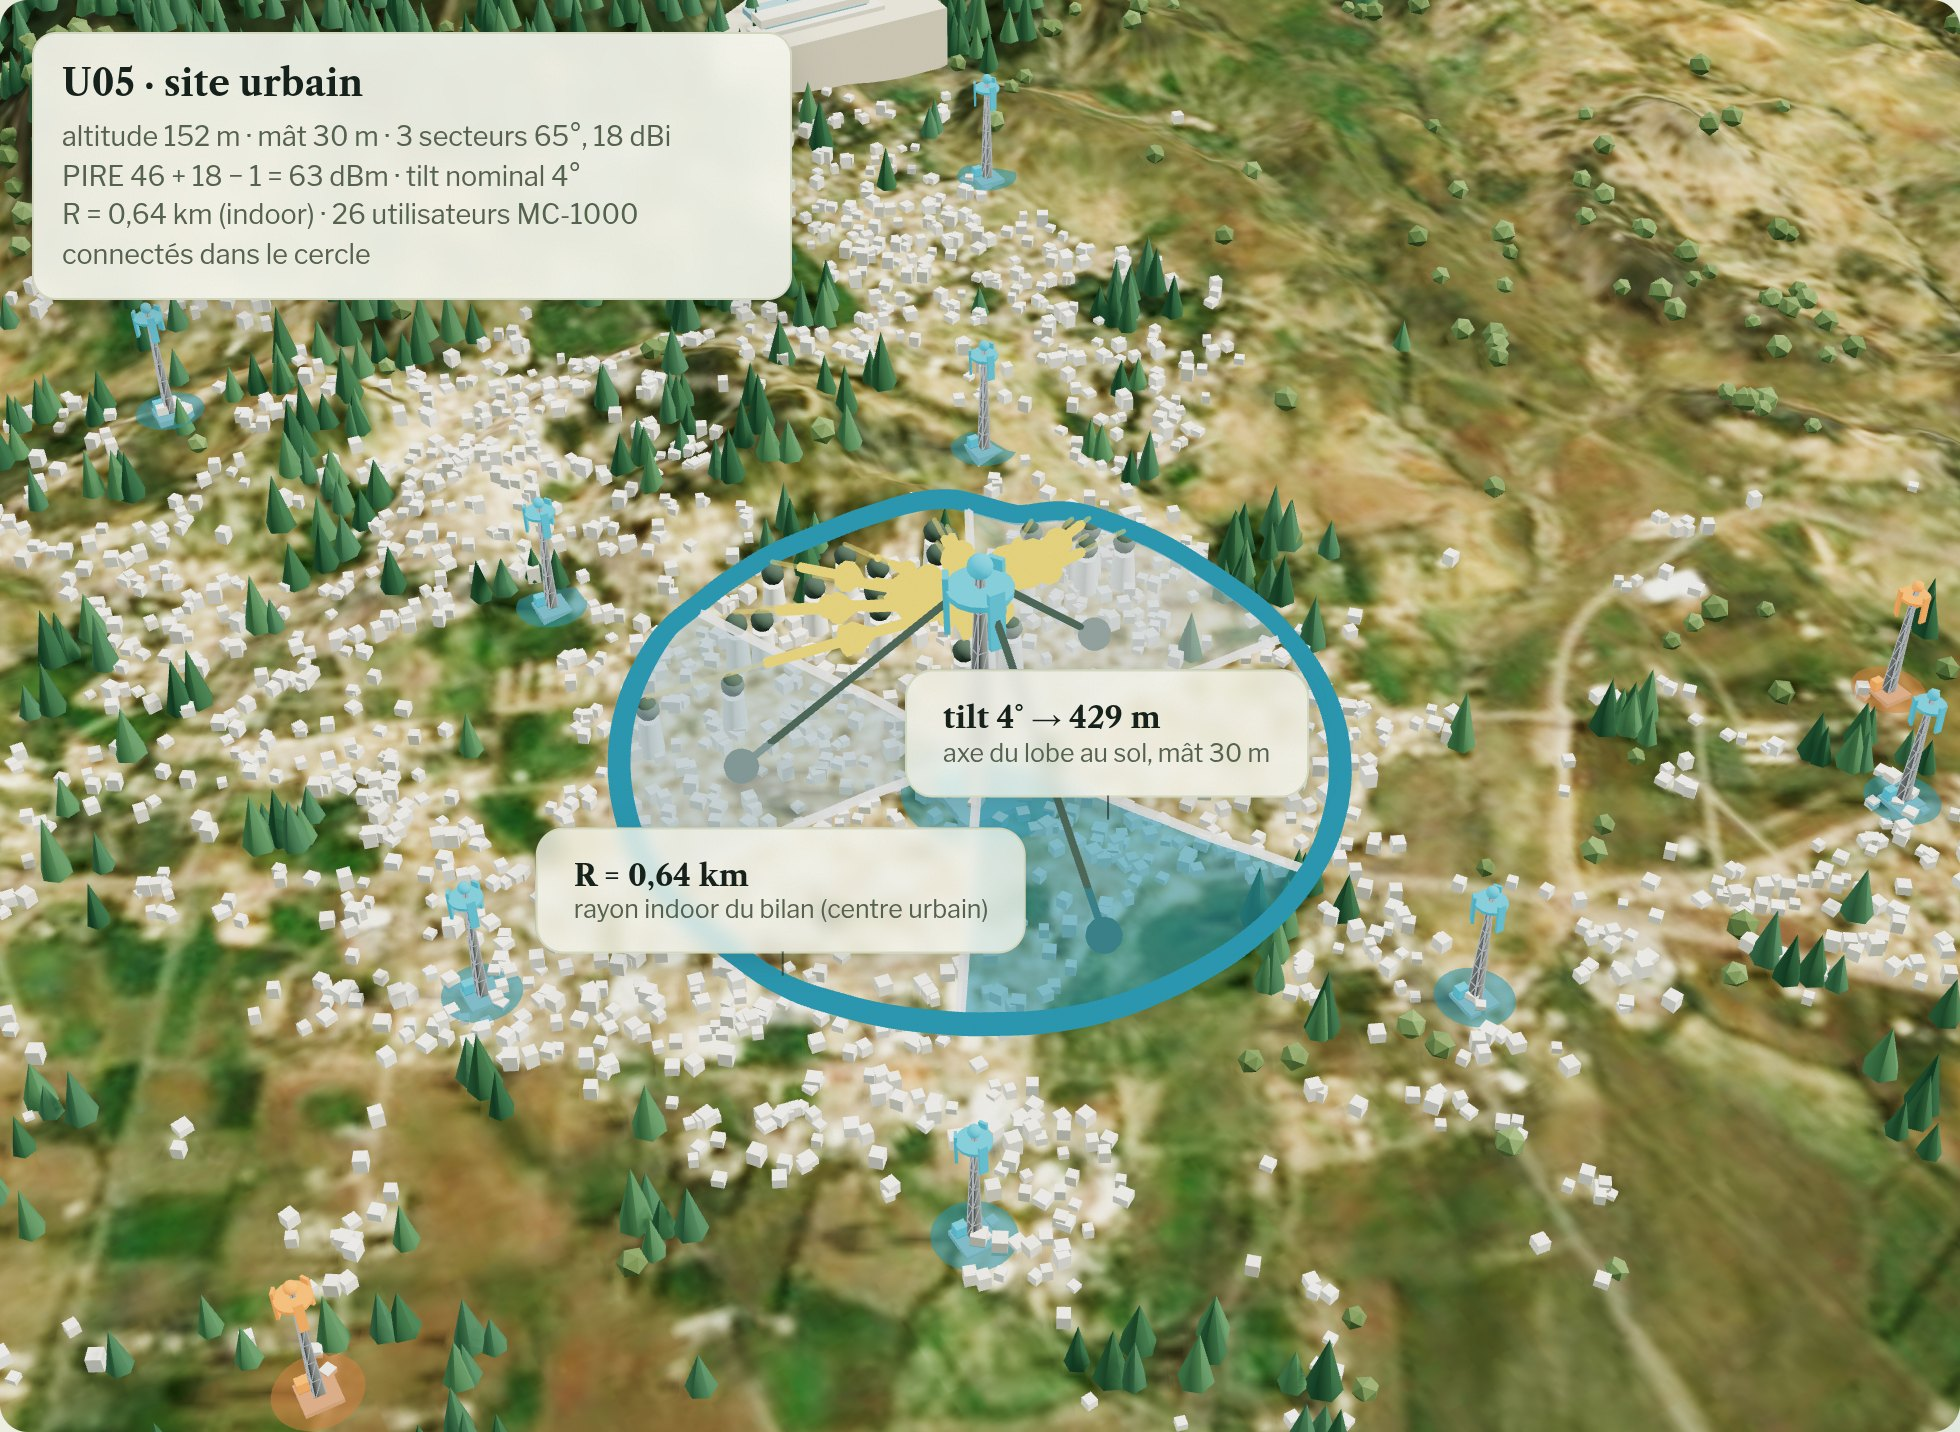
\includegraphics[width=\textwidth]{station-3d.jpg}\caption{Site U05 sur le terrain réel.}\end{subfigure}
\caption{Le site tri-sectoriel retenu.}
\label{fig-site}
\end{figure}

Sur la \cref{fig-site}b, le site U05 porte trois secteurs de \ang{65} ; le cercle a pour rayon $R = \SI{0,64}{\kilo\metre}$. Avec un tilt de \ang{4}, l'axe du lobe touche le sol à $30/\tan 4^\circ \approx \SI{430}{\metre}$.

\section{Dimensionnement par la capacité}
\label{sec-capa}

\subsection{Traduction de la logique GSM en LTE}

Le sujet décrit le dimensionnement par la capacité dans la logique GSM : fréquences par cellule, canaux de trafic égaux aux canaux totaux moins deux canaux de signalisation, abonnés par cellule par la loi d'Erlang~B, puis cellules et sites. Le LTE n'alloue pas de circuits mais des ressources temps-fréquence partagées. Nous gardons la même suite d'étapes en traduisant chaque notion (\cref{tab-gsm-lte}).

\begin{table}[H]
\centering
\caption{Étapes du sujet (GSM) et leur équivalent LTE.}
\label{tab-gsm-lte}
\begin{tabularx}{\textwidth}{@{}LLr@{}}
\toprule
\thead{Étape du sujet (GSM)} & \thead{Équivalent LTE} & \thead{Valeur} \\
\midrule
Fréquences par cellule & une porteuse de \SI{20}{\mega\hertz}, réutilisation 1 & 100 RB \\
Canaux de trafic = total $-$ 2 de signalisation & éléments de ressource (RE) par RB, moins le canal de contrôle (PDCCH) et les signaux de référence & DL 120/168 ; UL 144/168 \\
Abonnés par cellule (Erlang B, GoS) & débit de la cellule × charge maximale \SI{80}{\percent} / débit d'un abonné & 272 \\
Cellules = abonnés / abonnés par cellule & idem & 14 \\
Sites = cellules / 3 & idem (tri-secteur) & \textbf{5} \\
\bottomrule
\end{tabularx}
\end{table}

\begin{cours}{capacité d'un système cellulaire}
La capacité intrinsèque vaut $C_{\text{int}} = \dfrac{n}{K \cdot B}$, où $n$ est le nombre de canaux par porteuse, $K$ la taille du motif et $B$ la bande duplex d'un canal. En GSM ($n = 8$, $B = \SI{0,4}{\mega\hertz}$, $K = 9$), $C_{\text{int}} = 2{,}2$ canaux par cellule et par MHz. La capacité du réseau est $\dfrac{n\,\eta}{K \cdot B \cdot \pi R^2}$ en \si{Er\per\hertz\per\kilo\metre\squared}, où le rendement $\eta$ est le rapport entre canaux de trafic et canaux totaux~\cite{afif2026cours}.
\application Le rendement $\eta$ du cours est la ligne \enquote{canaux de trafic} du \cref{tab-gsm-lte}. Pour une porteuse GSM, $\eta = (8 - 2)/8 = 0{,}75$. En LTE, $\eta = 120/168 = 0{,}71$ en DL et $144/168 = 0{,}86$ en UL : la signalisation consomme une part comparable de la ressource. La formule montre aussi les deux leviers de capacité que nous utilisons : un motif $K$ petit (ici $K = 1$, \cref{sec-reuse}) et des cellules plus petites (rayon $R$).
\end{cours}

\subsection{Débit moyen d'une cellule}

Le débit d'une cellule dépend de la qualité de signal de ses utilisateurs. Nous avons appliqué la formule de C/I du cours (six interféreurs, \cref{sec-reuse}) en \emph{chaque point} d'une cellule hexagonale, converti chaque valeur en bearer Atoll grâce aux seuils de SINR, puis moyenné l'efficacité spectrale obtenue : \SI{1,894}{bit} par élément de ressource. Avec 120 RE utiles par RB et par milliseconde, 100 RB et le facteur applicatif de 0,95 d'Atoll,
\begin{equation}
  D_{\text{cellule}} = 1{,}894 × 120 × 100 × \num{1000} × 0{,}95 \approx \SI{21,6}{\Mbps} \text{ en DL}
\end{equation}
(\SI{25,9}{\Mbps} en UL). Le gain du MIMO, possible au-dessus de \SI{12}{\deci\bel} sur \SI{24}{\percent} de la cellule, n'est pas compté, ce qui rend l'estimation prudente.

\subsection{Demande et nombre de sites}

\begin{align}
  \text{abonnés LTE (centre)} &= \num{13590} × 0{,}939 × 0{,}30 × 0{,}93 \approx \num{3560}, \\
  \text{demande DL à l'heure chargée} &= \num{3560} × \SI{63,3}{\kbps} \approx \SI{225}{\Mbps}, \\
  \text{abonnés par cellule} &= \frac{\SI{21,6}{\Mbps} × 0{,}80}{\SI{63,3}{\kbps}} \approx 272, \\
  \text{cellules} &= \num{3560} / 272 \approx 13{,}1 \;\rightarrow\; 14, \qquad \text{sites} = 14 / 3 \;\rightarrow\; \mathbf{5}.
\end{align}
La capacité ne demande que 5 sites dans le centre, contre 11 pour la couverture indoor : la ville est aujourd'hui limitée par la couverture. Au rythme de croissance observé (+\SI{40}{\percent} en deux ans, soit $1{,}4^{5/2} \approx 2{,}3$ en cinq ans), le besoin en capacité atteindrait 11 sites dans cinq ans, ce que le réseau dimensionné par la couverture peut absorber. En campagne, la capacité demanderait 4 sites, contre 10 pour la couverture.

\section{Motif de réutilisation et plan de fréquences}
\label{sec-reuse}

\begin{cours}{réutilisation et rapport C/I}
Le nombre de cellules d'un motif vaut $K = i^2 + ij + j^2$ ($i$, $j$ entiers). La distance de réutilisation et le rapport de réutilisation co-canal sont
\begin{equation}
  D = \sqrt{3K}\,R, \qquad q = \frac{D}{R}.
\end{equation}
Avec $K_1$ cellules co-canal au premier anneau, $C \propto R^{-\alpha}$ et, pour un mobile en bord de cellule, $I_k \propto (D - R)^{-\alpha}$ :
\begin{equation}
  \frac{C}{I} = \frac{1}{\sum_{k=1}^{K_1} (q - 1)^{-\alpha}} = \frac{(q - 1)^{\alpha}}{6} \quad (K_1 = 6).
  \label{eq-ci}
\end{equation}
Seuils donnés dans le cours : \SI{18}{\deci\bel} en FDMA ; \SI{9}{\deci\bel} en GSM, d'où un motif de 7 ou 9 cellules ; \SI{3}{\deci\bel}, d'où un motif de 3 ou 4 cellules. Le système doit fonctionner avec le C/I le plus faible possible, pour réduire $D$ et la taille du motif~\cite{afif2026cours}.
\application L'indice du milieu $\alpha$ est la pente de notre modèle de Hata, $\alpha = 3{,}52$. Le seuil LTE est celui du bearer~4, \SI{-1}{\deci\bel}. Le \cref{tab-reuse} applique la formule~\eqref{eq-ci} à chaque motif.
\end{cours}

\begin{table}[H]
\centering
\caption{C/I dans le pire cas du cours selon le motif ($\alpha = 3{,}52$).}
\label{tab-reuse}
\small\setlength{\tabcolsep}{4.5pt}
\begin{tabular}{@{}ccccccc@{}}
\toprule
\thead{$K$} & \thead{$(i, j)$} & \thead{$q$} & \thead{C/I pire cas} & \thead{GSM ($\geq$ \SI{9}{\deci\bel})} & \thead{LTE ($\geq$ \SI{-1}{\deci\bel})} & \thead{Spectre par cellule} \\
\midrule
\rowcolor{mousse!50} \textbf{1} & (1, 0) & 1,73 & \SI{-12,6}{\deci\bel} & non & non & \textbf{\SI{20,0}{\mega\hertz}} \\
3 & (1, 1) & 3,00 & \SI{2,8}{\deci\bel} & non & oui & \SI{6,7}{\mega\hertz} \\
4 & (2, 0) & 3,46 & \SI{6,0}{\deci\bel} & non & oui & \SI{5,0}{\mega\hertz} \\
7 & (2, 1) & 4,58 & \SI{11,7}{\deci\bel} & oui & oui & \SI{2,9}{\mega\hertz} \\
9 & (3, 0) & 5,20 & \SI{14,2}{\deci\bel} & oui & oui & \SI{2,2}{\mega\hertz} \\
\bottomrule
\end{tabular}
\end{table}

Avec notre pente, nous retrouvons les ordres de grandeur du cours : le seuil GSM de \SI{9}{\deci\bel} conduit à $K = 7$ ou 9, et un seuil de \SI{3}{\deci\bel} à $K = 3$ ou 4. Pour le LTE (\SI{-1}{\deci\bel}), ce pire cas conduirait à $K = 3$. Il suppose cependant que l'utilisateur est en bord de cellule et que les six interféreurs sont tous au plus près en même temps. En calculant le C/I en chaque point de la cellule (\cref{fig-ci}), seuls \SI{8,4}{\percent} de la surface passent sous \SI{-1}{\deci\bel}, et la médiane est de \SI{5,4}{\deci\bel}. Comme le LTE adapte la modulation et le codage au SINR de chaque utilisateur, il tolère une qualité faible en bord de cellule. Nous retenons donc $K = 1$ : chaque cellule dispose des \SI{20}{\mega\hertz}, trois fois plus de spectre qu'avec $K = 3$. C'est la règle du cours (C/I le plus faible possible, donc motif le plus petit) appliquée jusqu'à $K = 1$ ; l'interférence en bord de cellule est ensuite traitée par la planification (tilt, azimut).

\begin{figure}[H]
\centering
\begin{subfigure}[b]{0.38\textwidth}\centering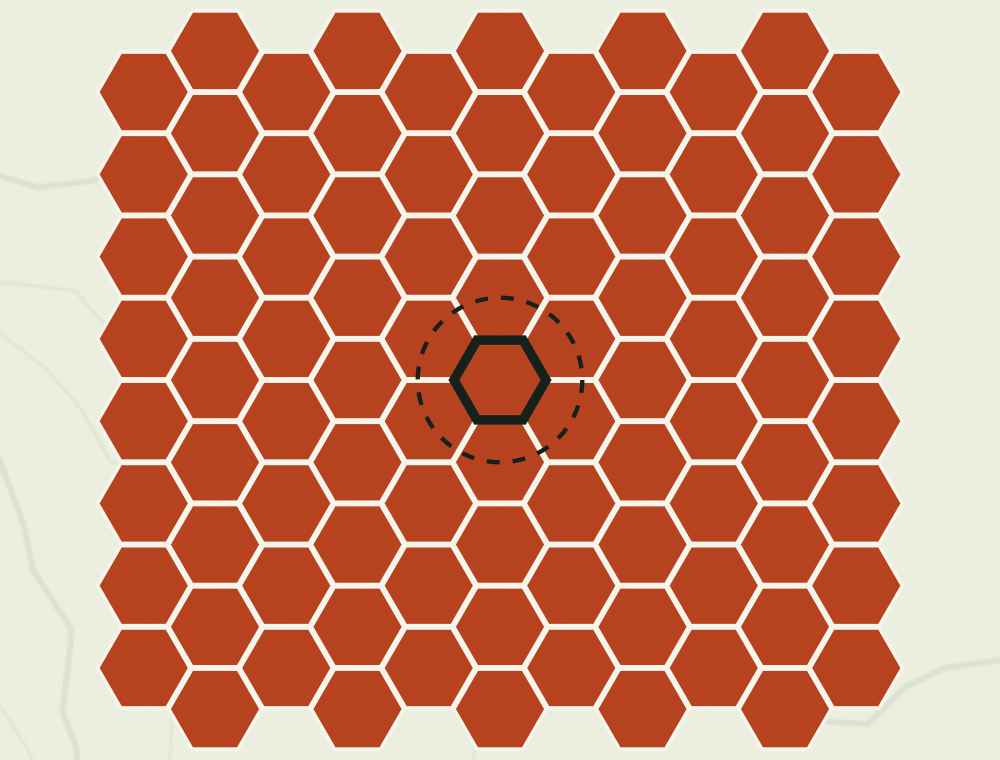
\includegraphics[width=\textwidth]{reuse-k1.png}\caption{Interféreurs co-canal, $K = 1$.}\end{subfigure}\hfill
\begin{subfigure}[b]{0.58\textwidth}\centering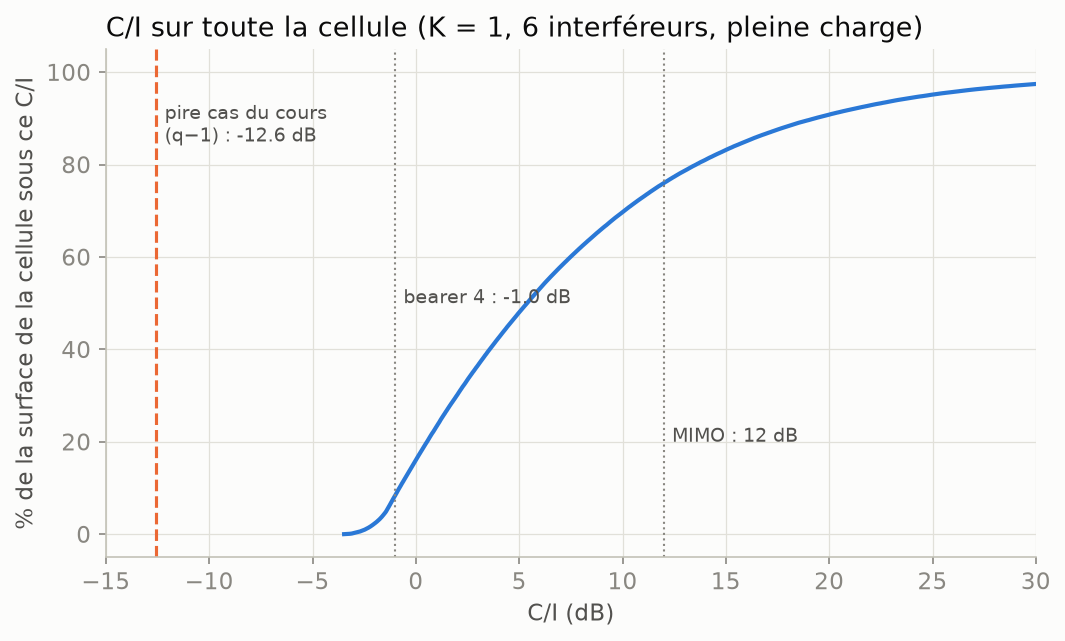
\includegraphics[width=\textwidth]{fig3_CI_cellule.png}\caption{C/I en chaque point de la cellule.}\end{subfigure}
\caption{C/I en réutilisation 1 : pire cas et distribution sur la cellule.}
\label{fig-ci}
\end{figure}

\paragraph{Plan de fréquences.} Toutes les cellules utilisent la même porteuse de \SI{20}{\mega\hertz} (EARFCN 1300, 100 RB). En LTE, la planification porte alors sur les identifiants physiques de cellule (PCI) : le site numéro $s$ reçoit les PCI $3s$, $3s + 1$ et $3s + 2$. Les trois secteurs d'un site ont ainsi des valeurs modulo 3 différentes, et leurs signaux de référence ne se superposent pas en fréquence~\cite{sesia2011}.

\section{Synthèse et choix de la bande}
\label{sec-800-1800}

\begin{table}[H]
\centering
\caption{Nombre de sites retenu par zone.}
\label{tab-sites-final}
\begin{tabular}{@{}lcccl@{}}
\toprule
\thead{Zone} & \thead{Couverture} & \thead{Capacité} & \thead{Retenu} & \thead{Contrainte} \\
\midrule
Centre urbain & 11 & 5 & 11 & couverture indoor \\
Rural & 10 & 4 & 10 & couverture outdoor \\
\midrule
\textbf{Total} & & & \textbf{21} & \\
\bottomrule
\end{tabular}
\end{table}

Dans chaque zone, le nombre retenu est le plus grand des deux besoins. Le même calcul a été mené à \SI{800}{\mega\hertz} (bande 20, \SI{10}{\mega\hertz}, modèle d'Okumura-Hata), avec les mêmes marges, les mêmes antennes et la même puissance par RB (\cref{tab-800-1800}).

\begin{table}[H]
\centering
\caption{Bandes 800 et \SI{1800}{\mega\hertz} comparées.}
\label{tab-800-1800}
\small\setlength{\tabcolsep}{5pt}
\begin{tabular}{@{}lccccc@{}}
\toprule
\thead{Bande} & \thead{$R$ urbain} & \thead{$R$ rural} & \thead{Sites\\couverture} & \thead{Total\\aujourd'hui} & \thead{Total dans\\5 ans} \\
\midrule
\SI{800}{\mega\hertz}, \SI{10}{\mega\hertz} & \SI{1,22}{\kilo\metre} & \SI{3,91}{\kilo\metre} & 6 & 12 & 24 \\
\SI{1800}{\mega\hertz}, \SI{20}{\mega\hertz} & \SI{0,64}{\kilo\metre} & \SI{2,06}{\kilo\metre} & 21 & 21 & \textbf{21} \\
\bottomrule
\end{tabular}
\end{table}

Le \SI{800}{\mega\hertz} demande moins de sites aujourd'hui (12 contre 21), car il porte plus loin. Avec \SI{10}{\mega\hertz} seulement, la ville y est limitée par la capacité (9 sites aujourd'hui), et il faudrait 24 sites dans cinq ans avec un trafic multiplié par 2,3. À \SI{1800}{\mega\hertz}, les 21 sites restent suffisants. Le \SI{800}{\mega\hertz} reste une bonne couche de couverture, que nous citons en perspective (\cref{ch-disc}).

\section{Le plan nominal}
\label{sec-nominal}

Les sites sont placés automatiquement sur une grille hexagonale de distance inter-sites $1{,}5\,R$ : \SI{0,96}{\kilo\metre} en ville et \SI{3,1}{\kilo\metre} en campagne, sans aucun site sur le massif. Les effets de bord donnent 20 sites (10 urbains, 10 ruraux) au lieu des 21 de la formule. Nous n'avons rien corrigé à la main : deux sites ruraux (R01, R02) tombent près de sites urbains et R07 tombe sur le flanc du massif. Ce plan brut est le réseau initial d'Atoll ; ses défauts sont corrigés au \cref{ch-opt}, avec une mesure avant et après chaque action.

\begin{figure}[H]
\centering
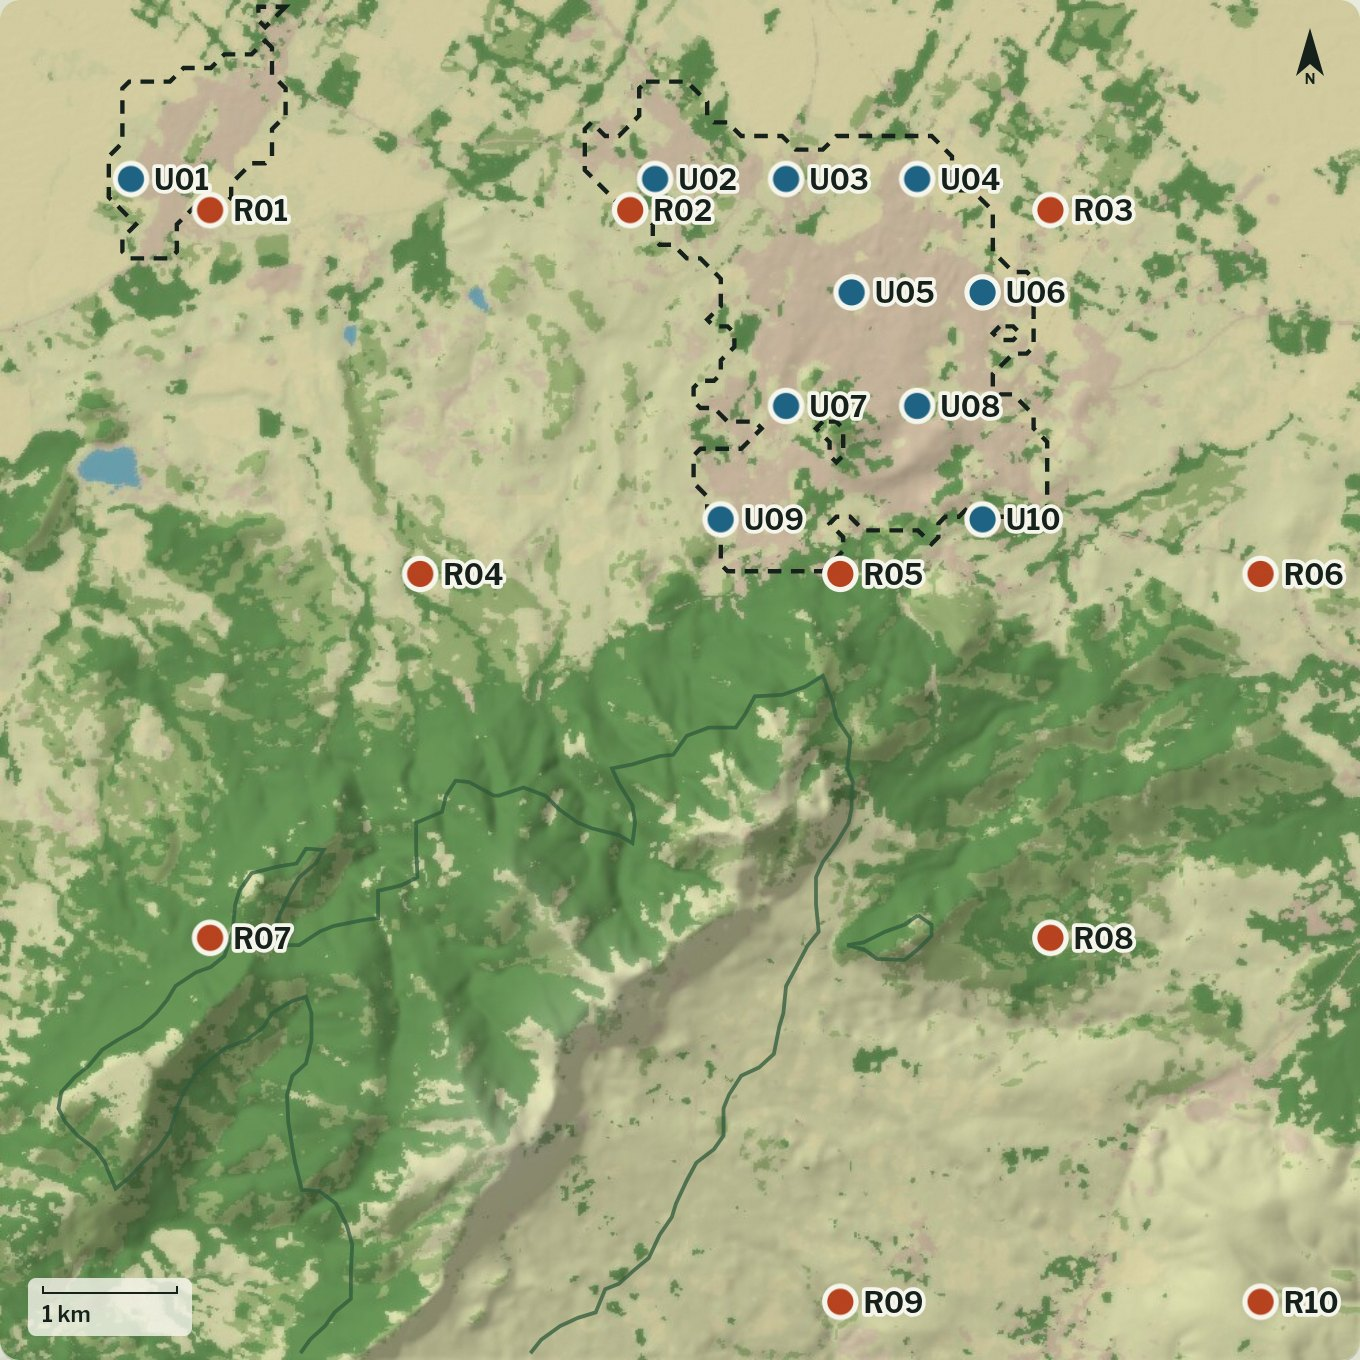
\includegraphics[width=0.6\textwidth]{plan-nominal.jpg}
\caption{Plan nominal (20 sites).}
\label{fig-nominal}
\end{figure}

Sur la \cref{fig-nominal}, les sites urbains sont en bleu et les sites ruraux en terre cuite ; leurs coordonnées sont données en \cref{ann-sites}.

\begin{retenir}
Le bilan de liaison donne un rayon de \SI{0,64}{\kilo\metre} en ville et \SI{2,06}{\kilo\metre} en campagne, limité par la liaison montante. La couverture impose 21 sites tri-sectoriels ; la capacité n'en demanderait que 5 dans le centre. La réutilisation retenue est $K = 1$, avec une porteuse de \SI{20}{\mega\hertz}.
\end{retenir}
